\documentclass[bigger]{beamer}

\usepackage{booktabs}
\useinnertheme{rounded}
\usecolortheme{crane}
\setbeamerfont{block title}{size={}}

\title{Measuring Predictive Performance of User Models: The Details Matter}

\author{Radek Pel\'anek\\[10mm]
%Masaryk University Brno\\
%Czech Republic

\includegraphics[width=.3\linewidth]{al-logo}
}

\date{EvalUMAP 2017}
 
\begin{document}

\frame{\titlepage}

\begin{frame}
  \frametitle{Introduction}

  \begin{itemize}
  \item Have you ever used the RMSE metric?
  \item Have you ever used the AUC metric?
  \end{itemize}

  \bigskip

  How \emph{exactly} did you compute them?
\end{frame}

\begin{frame}
  \frametitle{Evaluation over Historical Data}

  \emph{common evaluation approach}

  \begin{itemize}
  \item model building
  \item data collection
  \item cross-evaluation methodology (train/test division)
  \item model fitting
  \item \alert{quantifying model quality by measuring predictive accuracy}
  \item comparison of model, interpretation of results
  \end{itemize}
\end{frame}

\begin{frame}
  \frametitle{Measuring Predictive Accuracy}

    \begin{block}{}
  \begin{center}
      \begin{tabular}{llllllll}
        \midrule
        prediction & 0.7 & 0.6 & 0.9 & 0.95 & 0.8 & 0.85 & \ldots \\
        outcome & 0 & 1 & 1 & 0 & 1 & 1 & \ldots \\
        \midrule
      \end{tabular}
    
      \medskip

      $\Downarrow$

      \medskip

      quality of predictions (RMSE, AUC, ...)
  \end{center}  
    \end{block}

    \medskip    

    this step:
    \begin{itemize}
    \item gets little attention
    \item can significantly influence results
    \item can be nontrivial to do properly
    \end{itemize}
\end{frame}

\begin{frame}
  \frametitle{Motivation}

  \begin{itemize}
  \item Deep knowledge tracing, Piech et al. NIPS 2015
    \begin{itemize}
    \item claims of large improvement in model performance as measured by AUC
    \end{itemize}
  \item How deep is knowledge tracing?, Khajan et al., EDM 2016
    \begin{itemize}
    \item the ``improvement'' caused to large degree by methodological
      differences in computation of AUC
    \end{itemize}
  \end{itemize}
\end{frame}

\begin{frame}
  \frametitle{RMSE and AUC Metrics}

  \begin{itemize}
  \item Root Mean Square Error (RMSE) 
    \begin{itemize}
    \item $\sqrt{\frac{1}{n} \sum_{i=1}^n (o_i - p_i)^2}$
    \item closely related to ``Brier score''
    \end{itemize}
  \item Area Under the ROC Curve (AUC)
    \begin{itemize}
    \item Receiver Operating Characteristics (ROC) curve
    \item relative ranking of predictions
    \item widely used in many domains, but also widely criticized
    \end{itemize}
  \end{itemize}
\end{frame}

\begin{frame}
  \frametitle{Averaging}

  \begin{center}
    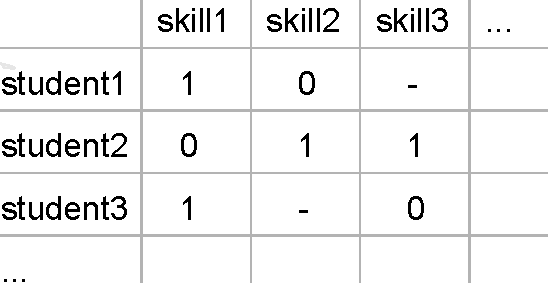
\includegraphics[width=.5\linewidth]{student-item-table}
  \end{center}

  %student modeling: skill $\times$ students data

  metric computation:
  \begin{itemize}
  \item global
  \item averaging across skills
  \item averaging across students
  \end{itemize}
\end{frame}

\begin{frame}
  \frametitle{Analysis of Student Modeling Literature}

  \begin{itemize}
  \item little attention to the choice of metric
  \item details of computation typically not specified
  \item AUC often used as a single metric
  \end{itemize}
\end{frame}

\begin{frame}
  \frametitle{Illustration of Metric Properties}

  \begin{itemize}
  \item scenarios with simulated data
  \item simple ``learning curve'' model of student behaviour
  \item illustration of metric properties
  \end{itemize}
\end{frame}

\begin{frame}
  \frametitle{Absolute Values of Metrics}

  \begin{block}{}
    Absolute values of metric do not express quality of models, but rather
    properties of data.
  \end{block}

  \medskip

  \begin{itemize}
  \item RMSE: baseline rate of events
  \item AUC: heterogeneity of data
  \end{itemize}

  \bigskip

\emph{Do not try to interpret the values.}

\emph{Do not compare values across data sets.}

\end{frame}

\begin{frame}
  \frametitle{Relative Values of Metrics}

  relative values = differences in metric values

  \begin{block}{}
    Very different models can have nearly the same metric value, particularly
    for AUC.
  \end{block}

  \bigskip

  \emph{Do not rely on AUC as a single metric to measure model performance.}  
\end{frame}

\begin{frame}
  \frametitle{Averaging Across Students}

  \begin{columns}   
    \begin{column}{.5\linewidth}
      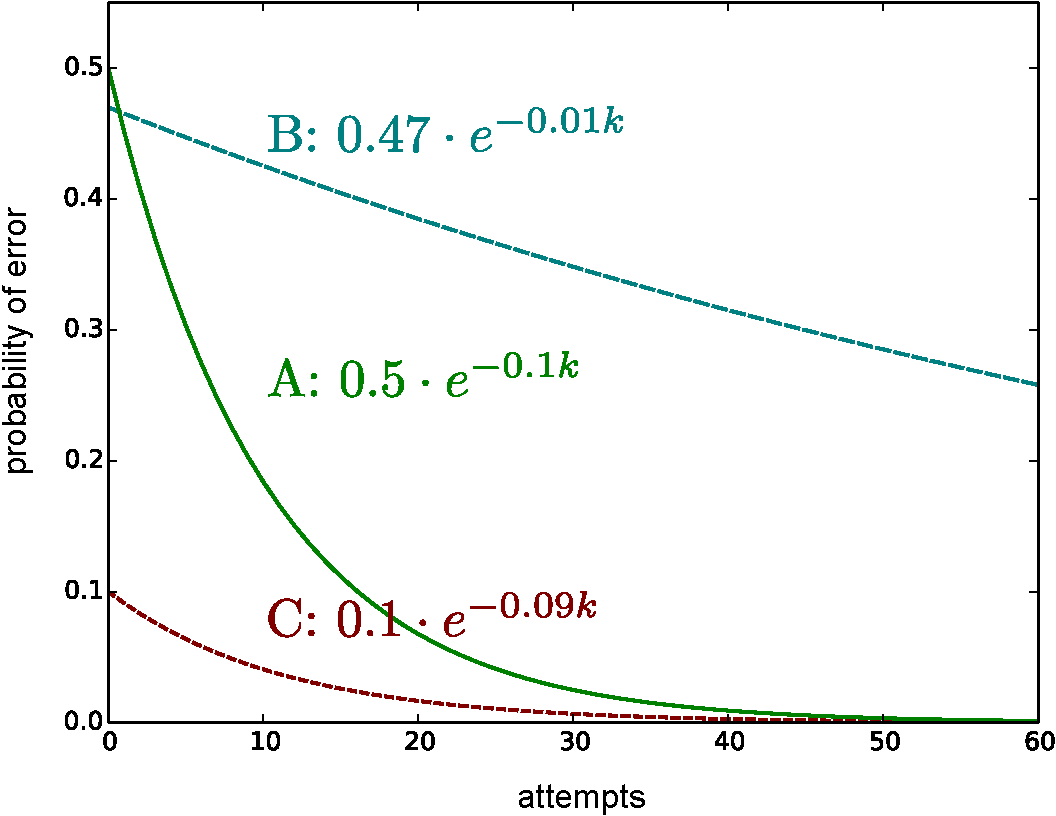
\includegraphics[width=\linewidth]{scenario-studentavg}

      \medskip

curve A\\
70\% of students: 5 attempts\\
30\% of students: 60 attempt
    \end{column}
    \begin{column}{.5\linewidth}
  \begin{tabular}{lll}
  \toprule
  model & RMSE & RMSE \\
  & global & per student \\
 \midrule
 B & 0.40 & 0.46 \\
 C & 0.35 & 0.48  \\
  \bottomrule  
\end{tabular}
    \end{column}
  \end{columns}
\end{frame}

\begin{frame}
  \frametitle{Averaging Across Skills}

  \begin{center}
    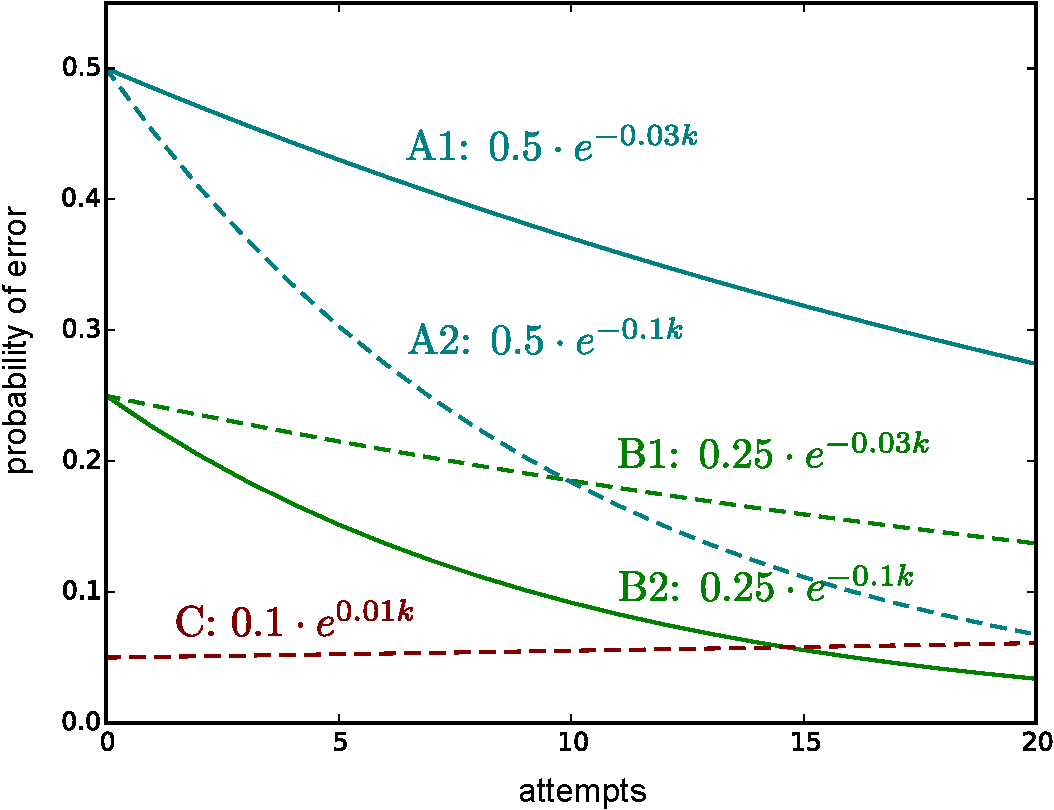
\includegraphics[width=.5\linewidth]{scenario-skillavg}

    \medskip
    \begin{tabular}{lll}
      \toprule
      model & AUC & AUC \\
      & global & per skill \\
      \midrule
      A1, B2 (correct) & 0.73  & 0.63 \\
      A2, B1 (speed mismatch) & 0.60 & 0.63 \\
      A1, C (negative learning) & 0.68  &  0.45 \\
      \bottomrule  
    \end{tabular}
  \end{center}
\end{frame}

\begin{frame}
  \frametitle{Summary}

  \begin{itemize}
  \item choice of metric matters
  \item details of metric computation matter
  \item should we adopt standards?
    \begin{itemize}
    \item ``universal metric'' -- no
    \item ``good practice'' -- yes
    \end{itemize}
  \end{itemize}
\end{frame}

\end{document}
